%%%%%%%%%%%%%%%%%%%%%%%%%%%%%%%%%%%%%%%%%%%%%%%%%%%%%%%%%%%%%%%%%%%%%%%%%%%%%%%
%% Electrochemical OER Application
%%
%% TODO: Put (s) on a-IrO3 phase in bulk Pourbaix diagram
%%%%%%%%%%%%%%%%%%%%%%%%%%%%%%%%%%%%%%%%%%%%%%%%%%%%%%%%%%%%%%%%%%%%%%%%%%%%%%%


% ################################# Paragraph #################################
% %%%%%%%%%%%%%%%%%%%%%%%%%%%%%%%%%%%%%%%%%%%%%%%%%%%%%%%%%%%%%%%%%%%%%%%%%%%%%
% TEMP
% %%%%%%%%%%%%%%%%%%%%%%%%%%%%%%%%%%%%%%%%%%%%%%%%%%%%%%%%%%%%%%%%%%%%%%%%%%%%%
% Short introduction into the cataylsis section
In the following section we will demonstrate the merit of our stable polymorph discovery algorithm by elucidating the electrochemical properties of the four promising structures discussed in the previous section.
In particular, surfaces constructed from the four polymorphs will be evaluated for their activity towards the oxygen evolution reaction (OER), an important chemistry with direct application to fuel cell devices.
Additionally, the surfaces will be evaluated for their stability and equilibrium surface coverage of surface oxygen and hydroxides.

% | - Bulk Pourbaix
\subsubsection{Bulk Pourbaix}

% ################################# Paragraph #################################
% %%%%%%%%%%%%%%%%%%%%%%%%%%%%%%%%%%%%%%%%%%%%%%%%%%%%%%%%%%%%%%%%%%%%%%%%%%%%%
% #COMBAK
% #QUESTION Use E or U for potential variable
% %%%%%%%%%%%%%%%%%%%%%%%%%%%%%%%%%%%%%%%%%%%%%%%%%%%%%%%%%%%%%%%%%%%%%%%%%%%%%
The electrochemical stability phase diagram (E vs. pH) was constructed by considering the equilibrium conditions of the following species: Ir, \rIrOtwo, \aIrOthree,  \rIrOthree, \bIrOthree, and an aqueous dissolved \ce{IrO[4-]} species (See TEMP|SI for additional details).
The resulting diagram is shown in Fig. \ref{fig:bulk_pourbaix}.
Importantly, under acidic conditions (pH \textless 7) and in the bias region of interest for the OER (~1.23 V vs. RHE) \aIrOthree shows a large window of stability.
This indicates that the \aIrOthree phase may be stabilized under the highly oxidizing conditions of the OER.
For comparison, the stability regions of the metastable \rIrOthree and \bIrOthree phases, in the absence of any other competing \ce{IrO_3} polymorphs, are indicated by unfilled solid lines.
As shown, these metastable phases appear to also have a wide region of stability in the OER region,
due to to their formation energies being within TEMP eV of the globally stable \aIrOthree phase, see SI table TEMP for the bulk energies of all considered phases.
Because of their similar energies it is possible that some or all of these \ce{IrO_3} phases may be present and relevent for the OER.
In the next section, we explore this possibility by computing the theoretical OER activity of these polymorph systems.
% Also explain the Ir and IrO[4-] ion

% | - Figure | Bulk Pourbaix Diagram
\begin{figure*}
\centering
\makebox[\textwidth][c]{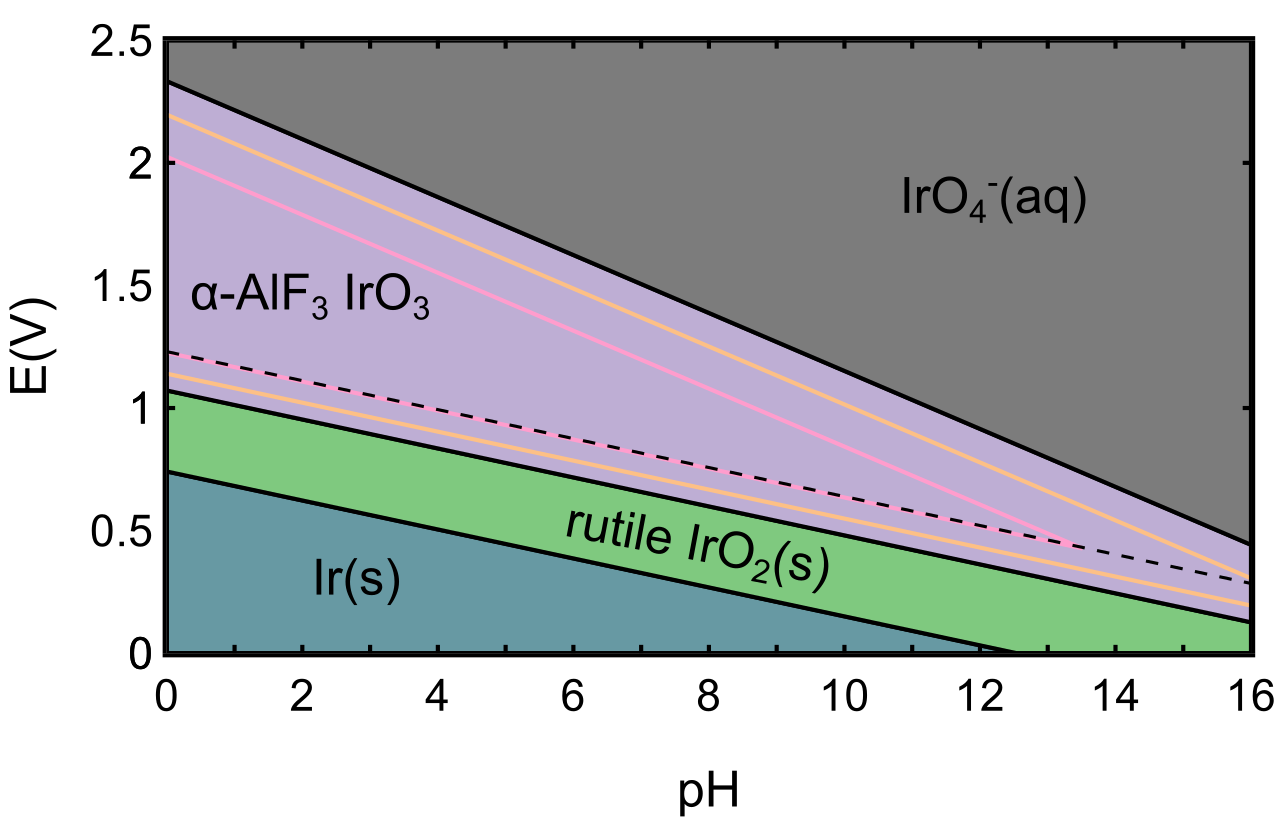
\includegraphics
{02_figures/oer_activity_stability/00_master__bulk-pourbaix__v1__400dpi__0__outplot.png}
% {02_figures/oer_activity_stability/bulk_pourbaix_0.pdf}
}
\caption{\label{fig:bulk_pourbaix},
Electrochemical bulk phasetability diagram (Pourbaix) of the Ir-O-H chemical space with respects to changes in potential and pH.
We considered a bulk unoxidized Ir(s) (blue), a [+4] \rIrOtwo  (green), and an aqueously dissolved \ce{IrO4[4-]} (grey) phase.
Additionnally, we considered the three \ce{IrO_3} polymorphs, \aIrOthree (purple), \rIrOthree (orange), and \bIrOthree (pink).
The water equilibrium line at 1.23 V vs RHE, which corresponds to a 0 overpotential catalyst, is shown by a dotted line.
}
\end{figure*}
% __|

% __|

% | - OER Activities and Surfaces
\subsubsection{b. OER Activities and Surfaces}

% ################################# Paragraph #################################
% %%%%%%%%%%%%%%%%%%%%%%%%%%%%%%%%%%%%%%%%%%%%%%%%%%%%%%%%%%%%%%%%%%%%%%%%%%%%%
% Introduction to OER results
% %%%%%%%%%%%%%%%%%%%%%%%%%%%%%%%%%%%%%%%%%%%%%%%%%%%%%%%%%%%%%%%%%%%%%%%%%%%%%
Fig. \ref{fig:oer_volcano} summarizes the major results of the electrochemical activity and surface stability analysis.
First, Fig. \ref{fig:oer_volcano} a.) shows the surace energy Pourbaix plots for the four IrOx crystals of interest. For each bulk system, the surface energy as a function of applied potential (pH=0), for various facets, and at various coverages (bare, *OH, and *O covered), are shown, see SI for more details.
% How facets were chosen | TODO Get x-ray pattern for systems
% TODO #REF | Reference for VESTA x-ray diff. pattern method
The specific facets were chosen from the highest intensity x-ray diffraction peaks from powder-diffraction spectra simulated in VESTA,
as well as using physical intuition as to which facets would be most physical.
% Say that the IrO3 bulk phase corresponds to the o-covered regime
Additionally, the bulk phase limits of stability from figure TEMP are included at the bottom of each subplot.
In most cases, the oxygen covered surfaces dominate at the OER equilibrium potential (1.23 V vs RHE) with bare surfaces being competitive to within TEMP eV/A2,
this competitivness goes away at even modest overpotentials (eta~0.3, --> ~1.5 V vs RHE),
at which point the oxygen covered terminations are further overstabalized relative to the bare surfaces,
making them the sole dominant termination.
% COMBAK, Revise "mainly" if we include some different coverags
Therefore in our activity analysis we consider mainly oxygen terminated surfaces for the OER.
The OER activity (expressed in terms of the limiting potential) for select oxygen terminated surfaces are shown in Fig. \ref{fig:oer_volcano} as a function of the DGO-DGOH TEMP OER thermodynamic descriptr.
The two rutile-IrO2 suraces (100, and 110) are located towards the strong binding side of the volcano, indicating that that they bind OER intemediate too strongly.
% Reference all experimental IrO2 overpotentials I can find
Encourangly, with predicted overpotentials of TEMP and TEMP, our rutile-IrO2 are within the range of experimental overpotentials found in literature.
The three IrO3 polymorph surfaces all have DGO-DGOH descriptor towards the top and right of the volcano, indicative of weaker binding energetics.
This is evident from figure SI TEMP (scaling) which shows a clear distinction between the IrO2 and IrO3 polymorphs, with IrO3 binding on average TEMP eV weaker than IrO2.
The best performing systems, including the (100), (110), and (211) facets of a-IrO3, b-IrO3 (101), and R-IrO3 (110), have overpotentials of ~0.4 V vs RHE,
a ~0.2 V vs RHE improvemnt over the rutile-IrO2 system.
We note that the computed  overpotentials for our \rIrOtwo system differs from that reported in REFERENCE_Colin_Science by ~0.2 V. This discrepency is due to our us of spin-polarization, which was neglected in Seitz et al., which strenghens the binding of IrO2.


% | - Figure | OER Volcano/Surface Pourbaix
\begin{figure*}
\centering
\makebox[\textwidth][c]{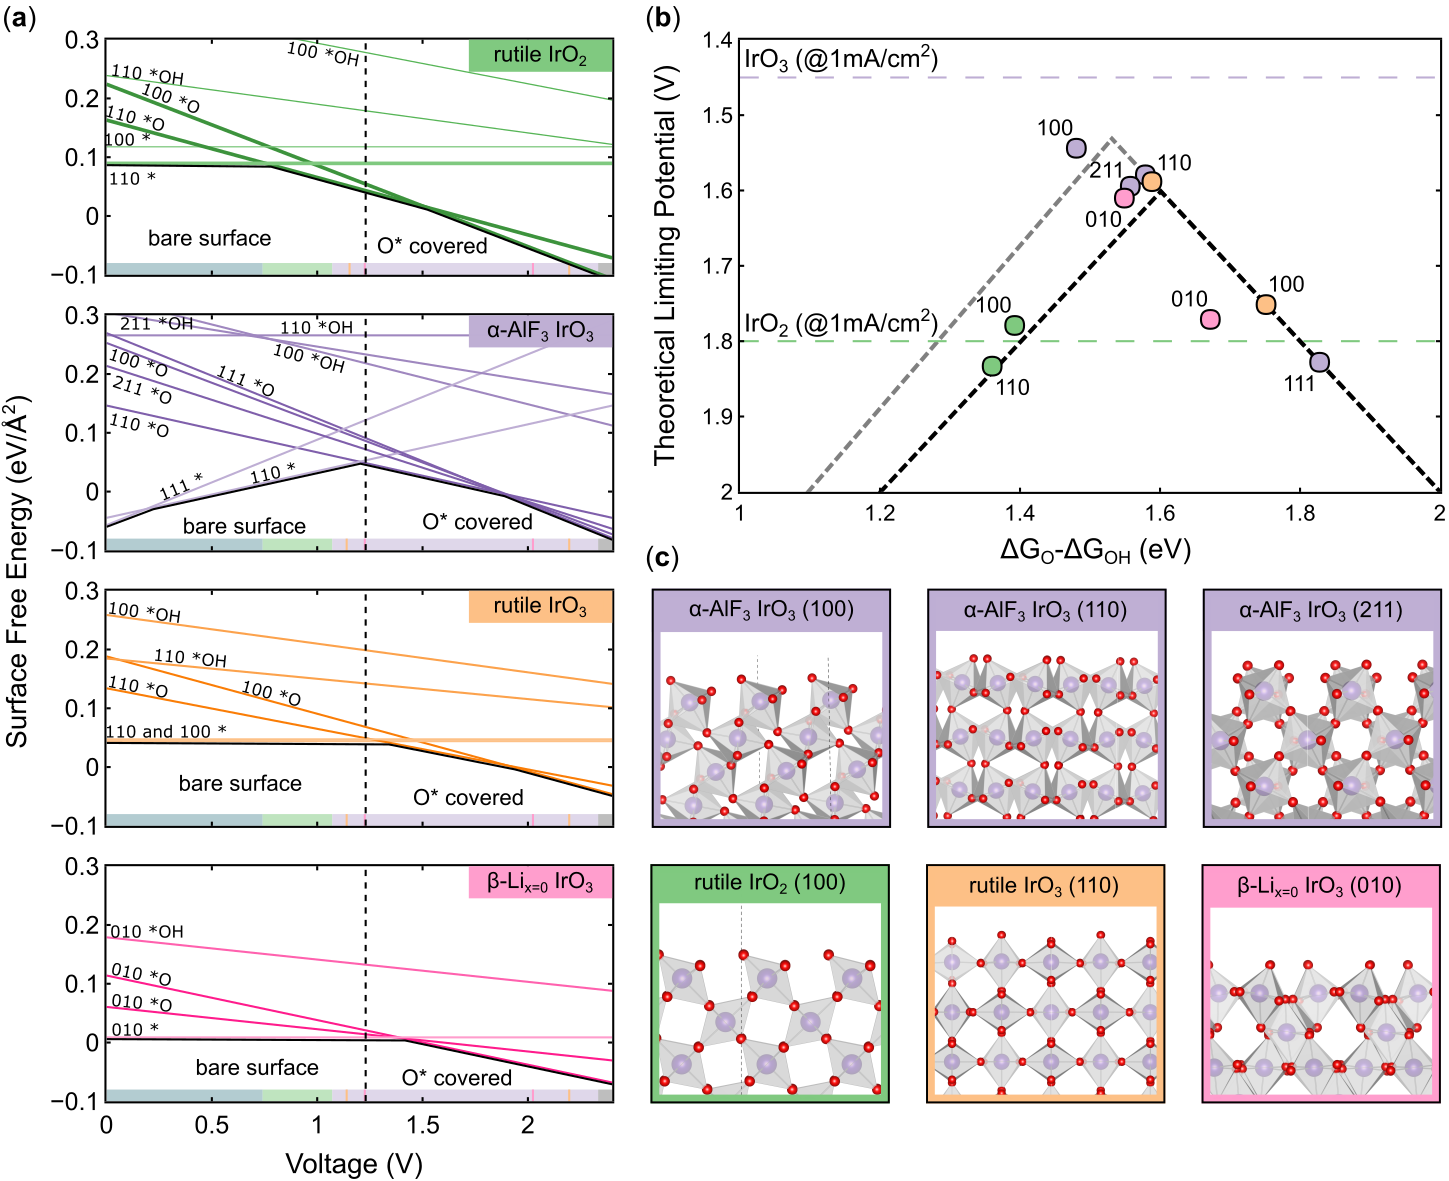
\includegraphics
{02_figures/oer_activity_stability/00_master__oer-volc_surf-pourb_struct__main_v3__200dpi__outplot.png}
% {02_figures/oer_activity_stability/00_master_plot__oer-volc_surf-pourb_struct__main_v3__outplot.pdf}
}
\caption{\label{fig:oer_volcano}
Summary of OER results for the four bulk structures of \IrOx considered: rutile-\ce{IrO_2} (green), $\alpha$-\ce{IrO_3} (purple), rutile-\ce{IrO_3} (orange), and $\beta$-\ce{IrO_3} (pink).
% -----------------------------------------------------------------------------
(a) Surface energy Pourbaix diagrams for each structure, with the surface energy of various facets and coverages shown as a function of applied potential.
The bulk Pourbaix diagram's bounds of stability at pH 0 are superimposed at the bottom of each subplot.
% -----------------------------------------------------------------------------
(b) OER activity volcano for \IrOx systems considered utilizing the \DGOmOH thermodynamic descriptor.
The purple dotted line corresponds to the experimental limiting potential at 10 mA cm\textsuperscript{2} for \ce{IrO_3}, % #TODO #REF Insert Seitz Science reference
while the green band corresponds to the range of experimentally observed overpotentials for pristine \ce{IrO_2} catalysts.  % TODO Insert green band into figure
% -----------------------------------------------------------------------------
(c) Select surface facets for the four \IrOx crystal systems considered.
% -----------------------------------------------------------------------------
% | - __old__
% Circles designate oxygen covered surfaces while triangles designate hydroxyl (*OH) terminated surfaces (relevant surface terminations were found via surface Pourbaix analyses).
% Surface energies at standard conditions (pH and V = 0) are reflected in the border color for each data point, where black indicates a low energy surface termination and white indicates more unstable surfaces.  % Currently not implemented as this
% The color range goes from x to y.
% __|
}
\end{figure*}
% __|

% __|

% | - OER Scaling Relations | TODO | MOVE THIS TO SI
\subsubsection{c. OER Intermediate Scaling}

% ################################# Paragraph #################################
% %%%%%%%%%%%%%%%%%%%%%%%%%%%%%%%%%%%%%%%%%%%%%%%%%%%%%%%%%%%%%%%%%%%%%%%%%%%%%
% TEMP
% %%%%%%%%%%%%%%%%%%%%%%%%%%%%%%%%%%%%%%%%%%%%%%%%%%%%%%%%%%%%%%%%%%%%%%%%%%%%%
Figure TEMP shows the scaling relations between the adsorption free energies of the OER intermediate species for the \IrOx systems studied herein.
It can be seen clearly that the data points corresponding to the three \ce{IrO_3} polymorphs are roughly 1 eV weaker binding than the rutile-\ce{IrO_2} points.
This generally weaker binding of the \ce{IrO_3} stoichiometry is responsible for the observed improvement in theoretical activity.
The \DGOOH vs.\DGOH relationship is very close to the traditional ``universal scaling relations'', demonstrating that our materials do not break the infamous \DGOOH vs. \DGOH scaling.

% | - Figure | OER Scaling Relations
\begin{figure*}
\centering
\makebox[\textwidth][c]{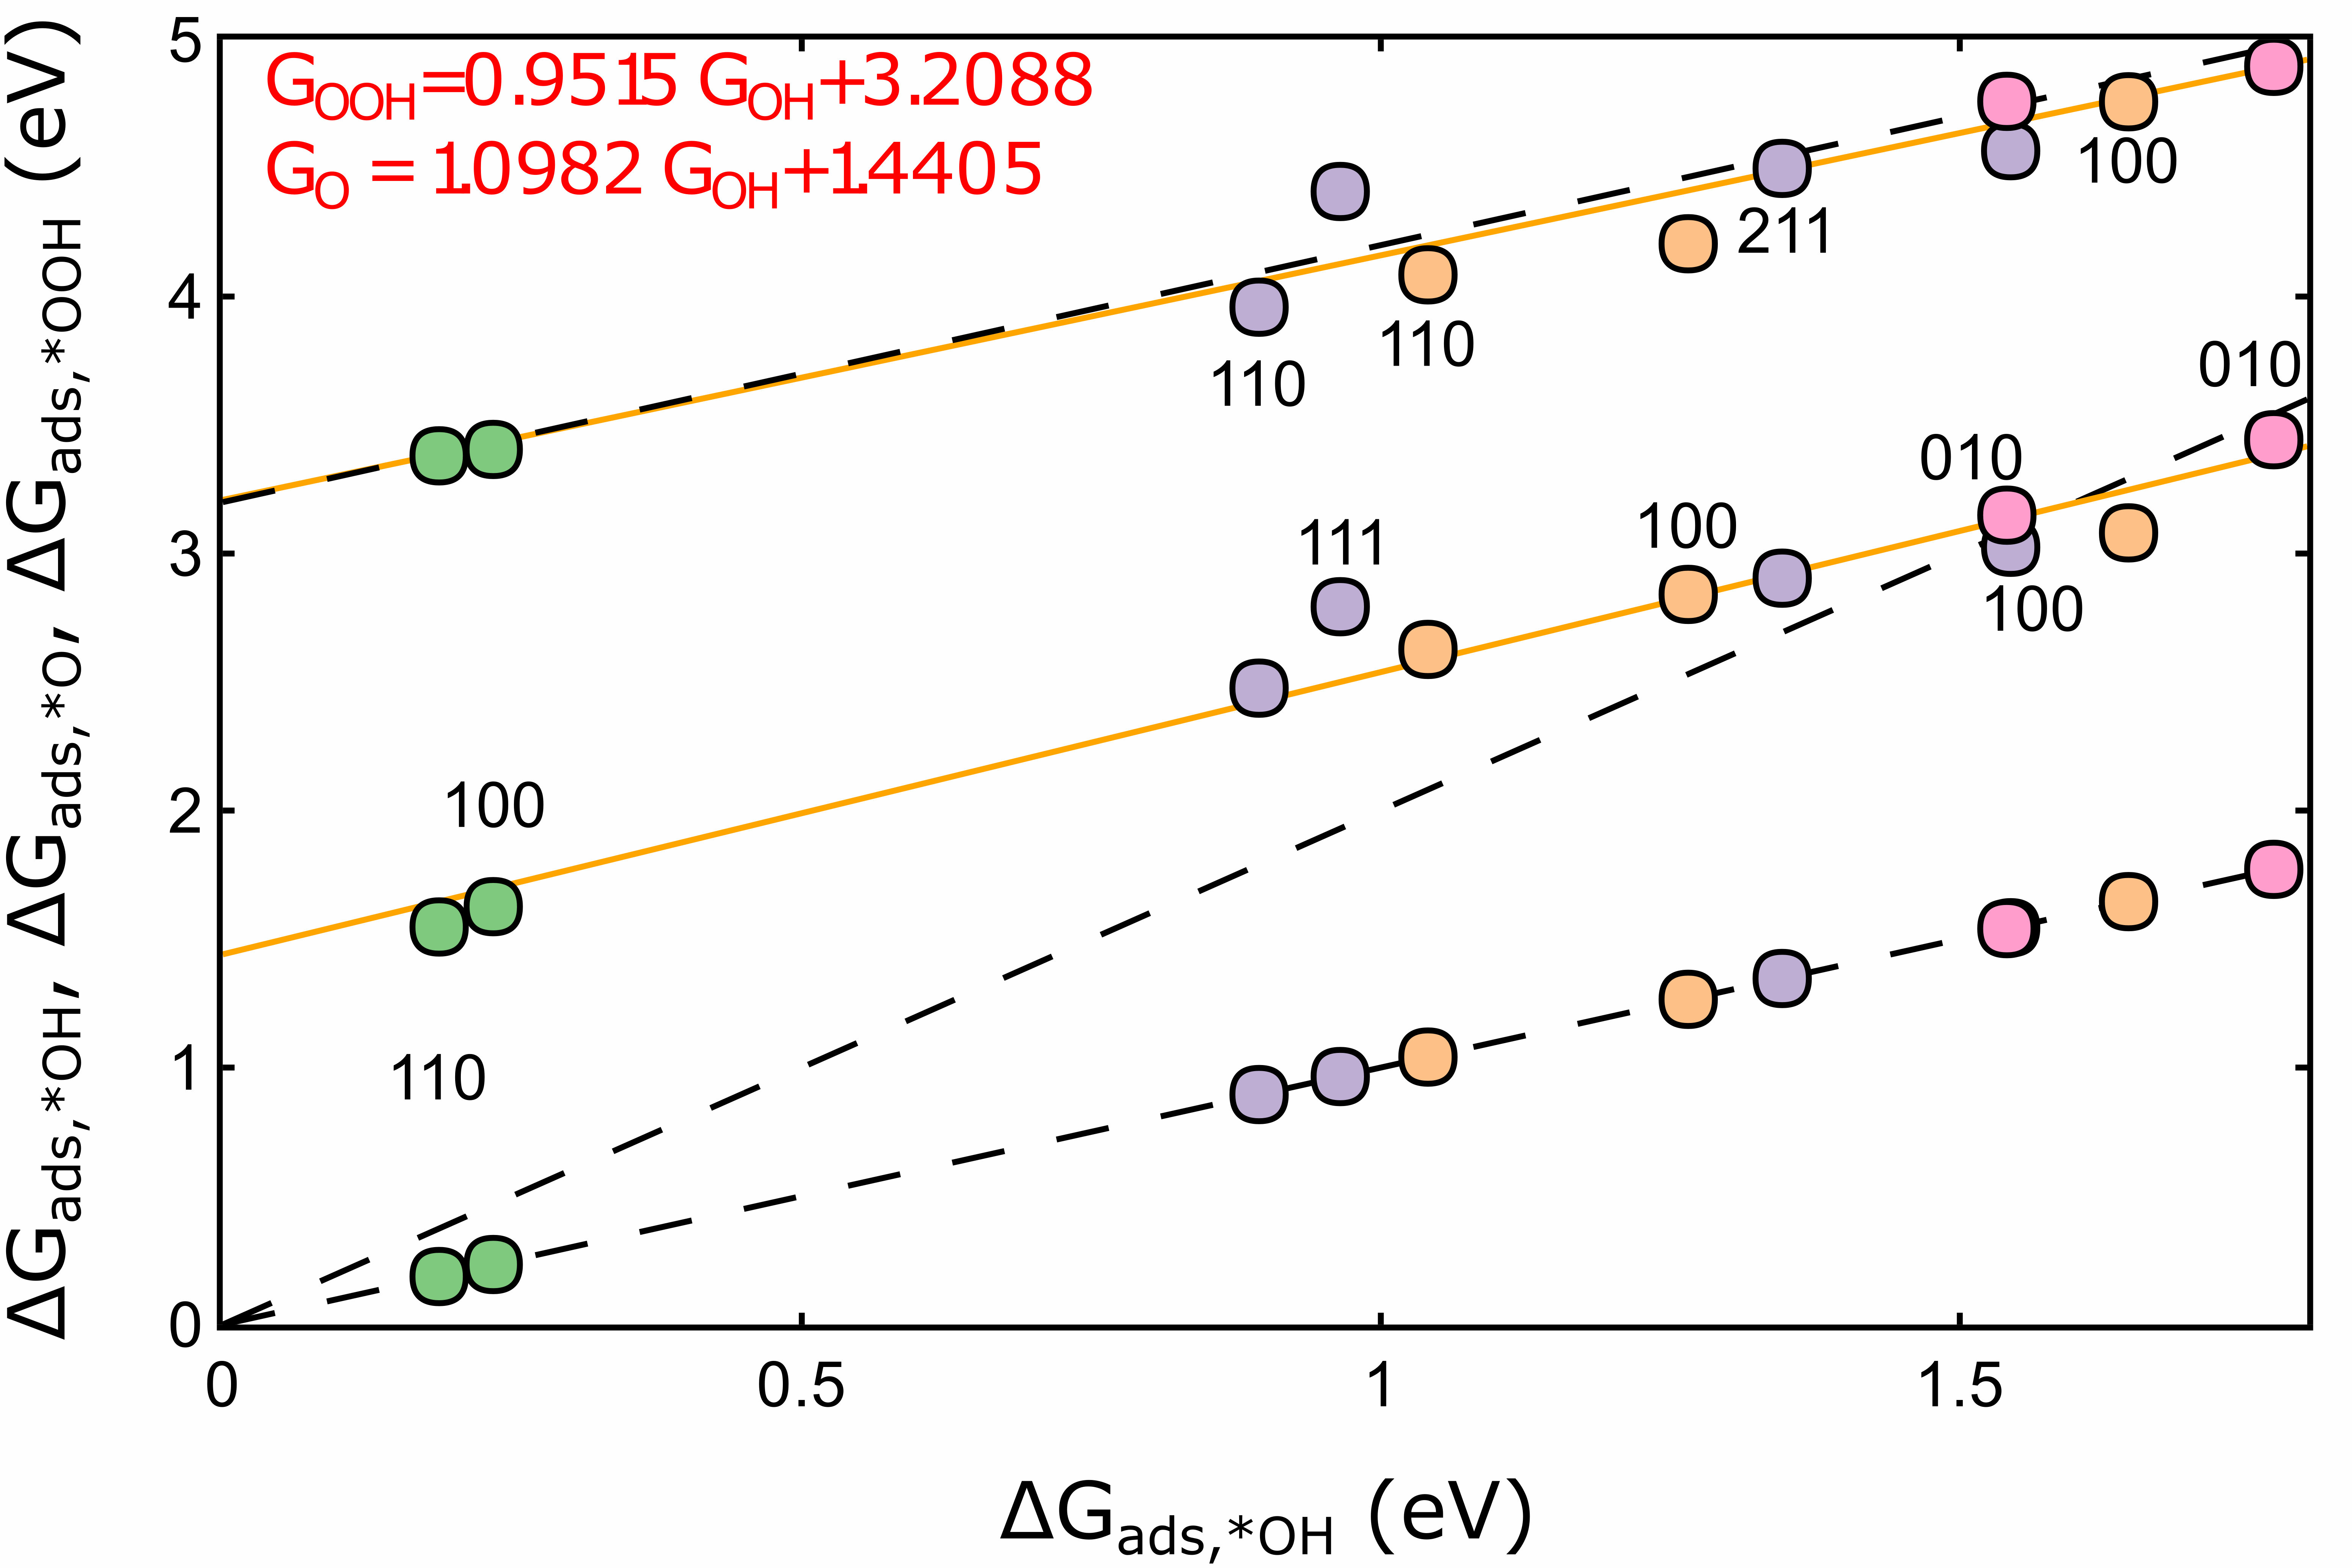
\includegraphics
{02_figures/oer_activity_stability/00_master__oer_scaling__main_v0__outplot2.png}
% {02_figures/oer_activity_stability/pl_scaling_relations_tmp.pdf}
}
\caption{\label{fig:scaling_relations}
% Adsorption free energy scaling relations plot.
Relationship between the adsorption free energies of the three key OER intermediates (*OH, *O, *OOH), with \DGOH chosen as the dependent variable.
Best fit lines are provided for \DGOOH vs. \DGOH and \DGO vs. \DGOH.
Additionally, ``universal scaling relations'' for \DGOOH vs. \DGOH and \DGO vs. \DGOH are shown (black dotted lines) to emphasize our deviation from the traditionally reported scaling fits.
The trivial \DGOH vs. \DGOH relationship is included for completeness.
% TODO Do I have to redefine the color convention every caption?
}
\end{figure*}
% __|

% __|
